\documentclass[12pt]{book}
\usepackage[utf8]{inputenc}
\usepackage{amsmath, amssymb, amsthm}  % For enhanced math formatting
\usepackage{enumitem}                  % Better control over itemize/enumerate
\usepackage{hyperref}   
\usepackage{graphicx}
\usepackage[normalem]{ulem}

\newtheorem{definition}{Definition}   % For theorems and definitions
\newtheorem{theorem}{Theorem}
\theoremstyle{definition}
\newtheorem{exmp}{Example}[section]   % Example environment, reset at each section

\title{Probability Theory Notes}
\author{Meow}

\setlength{\parindent}{1em} % Indentation for paragraphs

\begin{document}

\maketitle

\chapter{Probability}
\section{Set theory basics}
A set is a collection of objects. If \(S\) is a set, \(x \in S\) means that the element \(x\) is in the set \(S\):
\begin{itemize}
    \item \(\{1, 3, 5, 7, \dots \}\) is the set of all odd numbers.
    \item \(\mathbb{R}\) is the set of all real numbers.
    \item \([3, 7]\) is the set of all real numbers between 3 and 7.
\end{itemize}

The \textbf{empty set} is the smallest set, containing no elements, denoted by \(\emptyset\).
If \(A\) and \(B\) are sets and \(A \subseteq B\), it means that every element of \(A\) is in \(B\), expressed by:
\begin{equation}
    A \subseteq B \quad \text{if and only if} \quad \forall x \in A, x \in B.
\end{equation}

Two sets are equal if they have the same elements. The \textbf{union} of sets \(A\) and \(B\), denoted by \(A \cup B\), represents the set of all elements that are in \(A\) or \(B\), expressed by:
\begin{equation}
    A \cup B = \{ x \mid x \in A \text{ or } x \in B \}.
\end{equation}

Alternatively, using logical symbols, it can be written as:
\begin{equation}
    A \cup B = \{ x \mid x \in A \lor x \in B \}.
\end{equation}

The \textbf{intersection} of the sets \(A\) and \(B\), denoted by \(A \cap B\), represents the set of elements that they have in common, expressed by:
\begin{equation}
    A \cap B = \{ x \mid x \in A \text{ and } x \in B \}.
\end{equation}

The \textbf{complement} of \(A\), denoted by \(A^c\), represents the elements that are not in the set \(A\), expressed by:
\begin{equation}
    A^c = \{ x \mid x \notin A \}.
\end{equation}

We say that \(A\) and \(B\) are \textbf{disjoint} if they have no elements in common (their intersection is empty), denoted by \(A \cap B = \emptyset\). Two sets \(A\) and \(B\) are equal if both \(A \subseteq B\) and \(B \subseteq A\). The sets \(A_1, A_2, \dots, A_n\) are \textit{mutually disjoint} if:
\begin{equation}
    A_i \cap A_j = \emptyset \quad \text{for all} \quad i \neq j, \quad i, j = 1, 2, \dots
\end{equation}
In this case, we can express the union as:
\begin{equation}
    A_1 \cup A_2 \cup \dots \cup A_n = \sum_{j=1}^{n} A_j \quad \text{and for infinite sets,} \quad \bigcup_{j=1}^{\infty} A_j.
\end{equation}

Similarly, the intersection for \(n\) sets is written as:
\begin{equation}
    \bigcap_{i=1}^{n} A_i.
\end{equation}

The idea holds even when dealing with infinite sets.

The \textbf{difference} between sets \(A\) and \(B\) is defined as:
\begin{equation}
    A - B = \{ x \mid x \in A \text{ and } x \notin B \}.
\end{equation}

The \textbf{symmetric difference} \(A \Delta B\) is:
\begin{equation}
    A \Delta B = (A - B) \cup (B - A).
\end{equation}

\textbf{De Morgan's} laws give us a duality between unions and intersections:
\begin{itemize}
    \item \((A_1 \cup A_2 \cup \dots \cup A_n)^c = A_1^c \cap A_2^c \cap \dots \cap A_n^c\)
    \item \((A_1 \cap A_2 \cap \dots \cap A_n)^c = A_1^c \cup A_2^c \cup \dots \cup A_n^c\)
\end{itemize}

The first law says that not being in at least one of the \(A_n\)'s is the same as not being in every single one of them.

The second law says that not being in all of the \(A_n\)'s is the same as being outside at least one of the \(A_n\)'s.

A \textbf{partition} is a collection of subsets \(A_1, A_2, \dots, A_n\) of \(S\) such that the union of those sets is equal to \(S\) and \(A_i \cap A_j = \emptyset\) for \(i \neq j\).

\subsection{Sequences}
The sequence $\{A_n\}, \quad n = 1, 2, \dots$ is a \textbf{monotone sequence} of sets if:
\begin{enumerate}
    \item $A_1 \subseteq A_2 \subseteq A_3 \subseteq \dots$ ($A_n$ is increasing). We denote that by $A_n^{\uparrow}$.
    \item $A_1 \supseteq A_2 \supseteq A_3 \supseteq \dots$ ($A_n$ is decreasing). We denote that by $A_n^{\downarrow}$.
\end{enumerate}

We can represent the sequences below:
\begin{figure}[h!]
    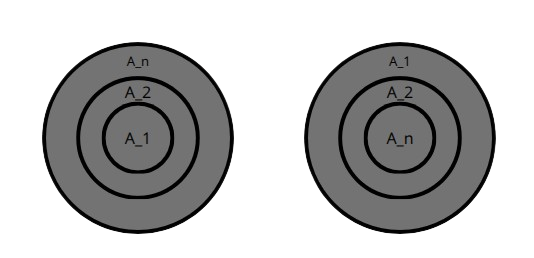
\includegraphics[width=\linewidth]{../assets/A_n.png}
\end{figure}

The \textit{limit} of the sequences is defined below:
\begin{enumerate}
    \item If it's increasing, then $\lim_{n \to \infty} A_n = \bigcup_{n = 1}^{\infty} A_n$
    \item If it's decreasing, then $\lim_{n \to \infty} A_n = \bigcap_{n = 1}^{\infty} A_n$
\end{enumerate}

Generally:
\begin{equation}
    \uline{A} = \liminf_{n \to \infty} A_n = \bigcup_{n = 1}^{\infty}\bigcap_{j = n}^{\infty} A_j
\end{equation}

and: 

\begin{equation}
    \bar{A} = \limsup_{n \to \infty} A_n = \bigcap_{n = 1}^{\infty}\bigcup_{j = n}^{\infty} A_j
\end{equation}

If these limits are equal, the sequence has a limit.

\end{document}
